\documentclass{standalone}
\usepackage{tikz}
\usetikzlibrary{patterns, positioning}


\begin{document}
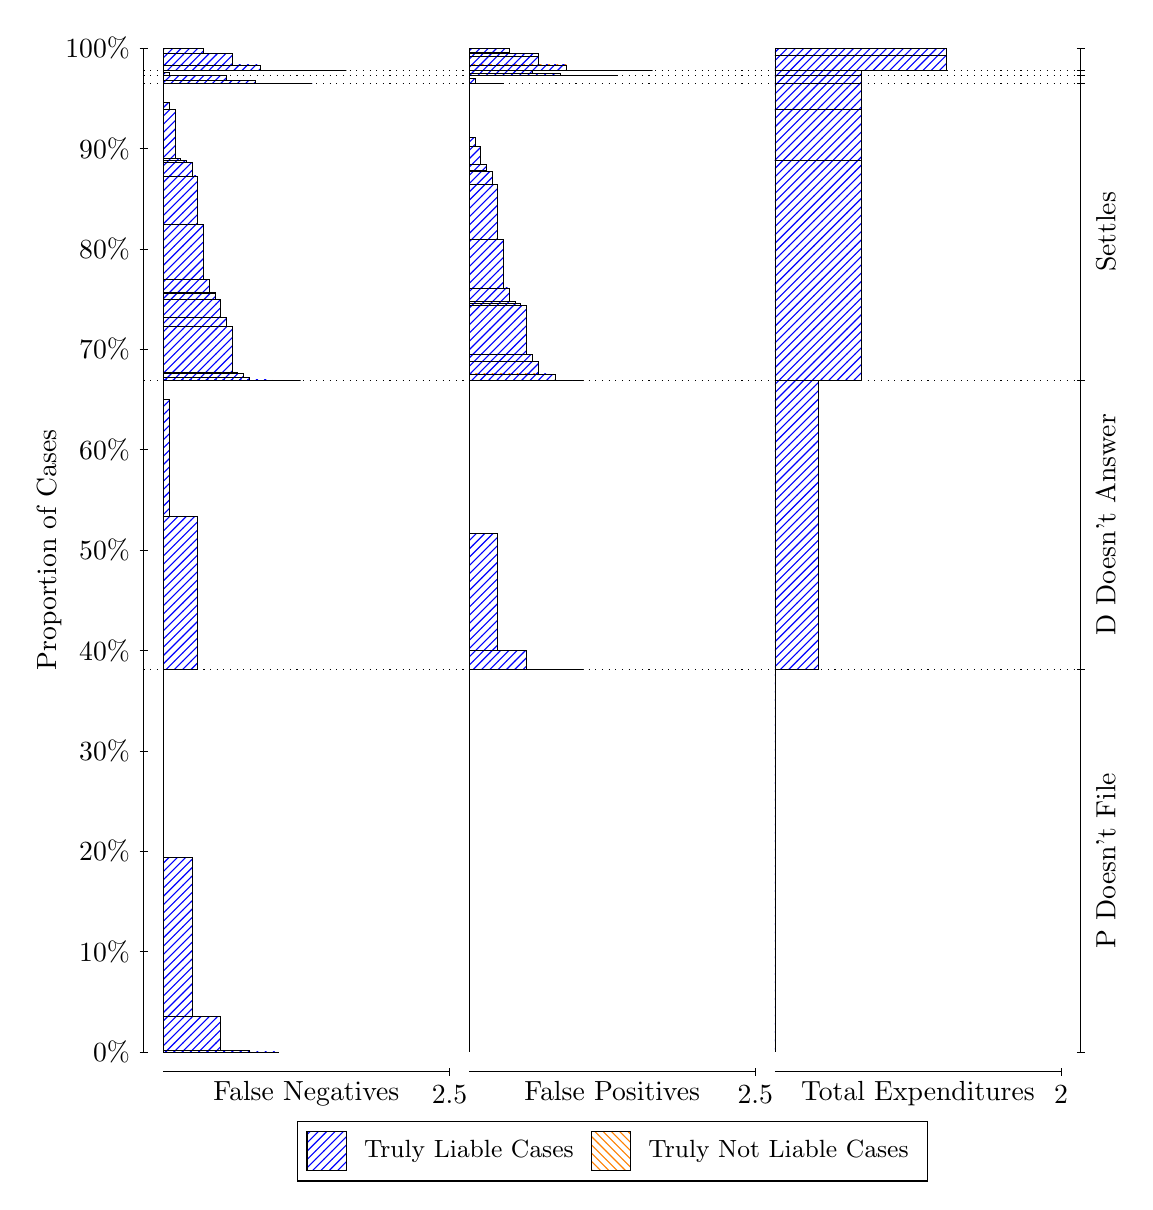
\begin{tikzpicture}
\draw[black, very thin] (1.5,1.75) -- (1.5,14.5);
\node[rotate=90, text=black, anchor=center] at (0.3, 8.125) {Proportion of Cases};
\draw[black, very thin] (1.45,1.75) -- (1.55,1.75);
\node[text=black, anchor=east] at (1.45, 1.75) {0\%};
\draw[black, very thin] (1.45,3.025) -- (1.55,3.025);
\node[text=black, anchor=east] at (1.45, 3.025) {10\%};
\draw[black, very thin] (1.45,4.3) -- (1.55,4.3);
\node[text=black, anchor=east] at (1.45, 4.3) {20\%};
\draw[black, very thin] (1.45,5.575) -- (1.55,5.575);
\node[text=black, anchor=east] at (1.45, 5.575) {30\%};
\draw[black, very thin] (1.45,6.85) -- (1.55,6.85);
\node[text=black, anchor=east] at (1.45, 6.85) {40\%};
\draw[black, very thin] (1.45,8.125) -- (1.55,8.125);
\node[text=black, anchor=east] at (1.45, 8.125) {50\%};
\draw[black, very thin] (1.45,9.4) -- (1.55,9.4);
\node[text=black, anchor=east] at (1.45, 9.4) {60\%};
\draw[black, very thin] (1.45,10.675) -- (1.55,10.675);
\node[text=black, anchor=east] at (1.45, 10.675) {70\%};
\draw[black, very thin] (1.45,11.95) -- (1.55,11.95);
\node[text=black, anchor=east] at (1.45, 11.95) {80\%};
\draw[black, very thin] (1.45,13.225) -- (1.55,13.225);
\node[text=black, anchor=east] at (1.45, 13.225) {90\%};
\draw[black, very thin] (1.45,14.5) -- (1.55,14.5);
\node[text=black, anchor=east] at (1.45, 14.5) {100\%};

\draw[black, very thin] (13.4,1.75) -- (13.4,14.5);
\draw[black, very thin] (13.35,1.75) -- (13.45,1.75);
\node[anchor=west] at (13.35, 1.75) {};
\draw[black, very thin] (13.35,6.6081) -- (13.45,6.6081);
\node[anchor=west] at (13.35, 6.6081) {};
\draw[black, very thin] (13.35,10.283) -- (13.45,10.283);
\node[anchor=west] at (13.35, 10.283) {};
\draw[black, very thin] (13.35,14.046) -- (13.45,14.046);
\node[anchor=west] at (13.35, 14.046) {};
\draw[black, very thin] (13.35,14.149) -- (13.45,14.149);
\node[anchor=west] at (13.35, 14.149) {};
\draw[black, very thin] (13.35,14.214) -- (13.45,14.214);
\node[anchor=west] at (13.35, 14.214) {};
\draw[black, very thin] (13.35,14.5) -- (13.45,14.5);
\node[anchor=west] at (13.35, 14.5) {};

\draw[black, very thin, pattern color=blue, pattern=north east lines] (1.75,1.75) rectangle (3.2033,1.7501);
\draw[black, very thin, pattern color=blue, pattern=north east lines] (1.75,1.7501) rectangle (2.84,1.7656);
\draw[black, very thin, pattern color=blue, pattern=north east lines] (1.75,1.7656) rectangle (2.4767,2.1981);
\draw[black, very thin, pattern color=blue, pattern=north east lines] (1.75,2.1981) rectangle (2.1133,4.2212);
\draw[black, very thin, pattern color=orange, pattern=north west lines] (1.75,4.2212) rectangle (1.75,4.2212);
\draw[black, very thin, pattern color=blue, pattern=north east lines] (1.75,4.2212) rectangle (1.75,6.6081);
\draw[black, very thin, pattern color=blue, pattern=north east lines] (1.75,6.6081) rectangle (2.186,8.5527);
\draw[black, very thin, pattern color=blue, pattern=north east lines] (1.75,8.5527) rectangle (1.8227,10.04);
\draw[black, very thin, pattern color=orange, pattern=north west lines] (1.75,10.04) rectangle (1.75,10.04);
\draw[black, very thin, pattern color=blue, pattern=north east lines] (1.75,10.04) rectangle (1.75,10.283);
\draw[black, very thin, pattern color=blue, pattern=north east lines] (1.75,10.283) rectangle (3.494,10.283);
\draw[black, very thin, pattern color=blue, pattern=north east lines] (1.75,10.283) rectangle (3.2033,10.283);
\draw[black, very thin, pattern color=blue, pattern=north east lines] (1.75,10.283) rectangle (3.1307,10.285);
\draw[black, very thin, pattern color=blue, pattern=north east lines] (1.75,10.285) rectangle (3.058,10.285);
\draw[black, very thin, pattern color=blue, pattern=north east lines] (1.75,10.285) rectangle (2.9127,10.285);
\draw[black, very thin, pattern color=blue, pattern=north east lines] (1.75,10.285) rectangle (2.84,10.316);
\draw[black, very thin, pattern color=blue, pattern=north east lines] (1.75,10.316) rectangle (2.7673,10.371);
\draw[black, very thin, pattern color=blue, pattern=north east lines] (1.75,10.371) rectangle (2.6947,10.379);
\draw[black, very thin, pattern color=blue, pattern=north east lines] (1.75,10.379) rectangle (2.622,10.962);
\draw[black, very thin, pattern color=blue, pattern=north east lines] (1.75,10.962) rectangle (2.5493,11.076);
\draw[black, very thin, pattern color=blue, pattern=north east lines] (1.75,11.076) rectangle (2.4767,11.306);
\draw[black, very thin, pattern color=blue, pattern=north east lines] (1.75,11.306) rectangle (2.404,11.387);
\draw[black, very thin, pattern color=blue, pattern=north east lines] (1.75,11.387) rectangle (2.404,11.399);
\draw[black, very thin, pattern color=blue, pattern=north east lines] (1.75,11.399) rectangle (2.3313,11.565);
\draw[black, very thin, pattern color=blue, pattern=north east lines] (1.75,11.565) rectangle (2.2587,12.261);
\draw[black, very thin, pattern color=blue, pattern=north east lines] (1.75,12.261) rectangle (2.186,12.875);
\draw[black, very thin, pattern color=blue, pattern=north east lines] (1.75,12.875) rectangle (2.1133,13.051);
\draw[black, very thin, pattern color=blue, pattern=north east lines] (1.75,13.051) rectangle (2.0407,13.071);
\draw[black, very thin, pattern color=blue, pattern=north east lines] (1.75,13.071) rectangle (2.0407,13.071);
\draw[black, very thin, pattern color=blue, pattern=north east lines] (1.75,13.071) rectangle (1.968,13.1);
\draw[black, very thin, pattern color=blue, pattern=north east lines] (1.75,13.1) rectangle (1.8953,13.717);
\draw[black, very thin, pattern color=blue, pattern=north east lines] (1.75,13.717) rectangle (1.8227,13.809);
\draw[black, very thin, pattern color=orange, pattern=north west lines] (1.75,13.809) rectangle (1.75,13.809);
\draw[black, very thin, pattern color=blue, pattern=north east lines] (1.75,13.809) rectangle (1.75,14.046);
\draw[black, very thin, pattern color=blue, pattern=north east lines] (1.75,14.046) rectangle (3.6393,14.046);
\draw[black, very thin, pattern color=blue, pattern=north east lines] (1.75,14.046) rectangle (3.276,14.046);
\draw[black, very thin, pattern color=blue, pattern=north east lines] (1.75,14.046) rectangle (2.9127,14.085);
\draw[black, very thin, pattern color=blue, pattern=north east lines] (1.75,14.085) rectangle (2.5493,14.148);
\draw[black, very thin, pattern color=blue, pattern=north east lines] (1.75,14.148) rectangle (2.186,14.149);
\draw[black, very thin, pattern color=orange, pattern=north west lines] (1.75,14.149) rectangle (1.75,14.149);
\draw[black, very thin, pattern color=blue, pattern=north east lines] (1.75,14.149) rectangle (2.186,14.15);
\draw[black, very thin, pattern color=blue, pattern=north east lines] (1.75,14.15) rectangle (1.8227,14.19);
\draw[black, very thin, pattern color=orange, pattern=north west lines] (1.75,14.19) rectangle (1.75,14.19);
\draw[black, very thin, pattern color=blue, pattern=north east lines] (1.75,14.19) rectangle (1.75,14.214);
\draw[black, very thin, pattern color=blue, pattern=north east lines] (1.75,14.214) rectangle (4.0753,14.214);
\draw[black, very thin, pattern color=blue, pattern=north east lines] (1.75,14.214) rectangle (3.712,14.215);
\draw[black, very thin, pattern color=blue, pattern=north east lines] (1.75,14.215) rectangle (3.3487,14.219);
\draw[black, very thin, pattern color=blue, pattern=north east lines] (1.75,14.219) rectangle (2.9853,14.285);
\draw[black, very thin, pattern color=blue, pattern=north east lines] (1.75,14.285) rectangle (2.622,14.429);
\draw[black, very thin, pattern color=blue, pattern=north east lines] (1.75,14.429) rectangle (2.2587,14.495);
\draw[black, very thin, pattern color=blue, pattern=north east lines] (1.75,14.495) rectangle (1.8953,14.5);
\draw[black, very thin, pattern color=orange, pattern=north west lines] (1.75,14.5) rectangle (1.75,14.5);
\draw[black, very thin, pattern color=blue, pattern=north east lines] (1.75,14.5) rectangle (1.75,14.5);
\draw[black, very thin, pattern color=orange, pattern=north west lines] (5.6333,1.75) rectangle (5.6333,1.75);
\draw[black, very thin, pattern color=blue, pattern=north east lines] (5.6333,1.75) rectangle (5.6333,6.6081);
\draw[black, very thin, pattern color=orange, pattern=north west lines] (5.6333,6.6081) rectangle (7.0867,6.6081);
\draw[black, very thin, pattern color=blue, pattern=north east lines] (5.6333,6.6081) rectangle (7.0867,6.6081);
\draw[black, very thin, pattern color=blue, pattern=north east lines] (5.6333,6.6081) rectangle (6.7233,6.6093);
\draw[black, very thin, pattern color=blue, pattern=north east lines] (5.6333,6.6093) rectangle (6.36,6.8514);
\draw[black, very thin, pattern color=blue, pattern=north east lines] (5.6333,6.8514) rectangle (5.9967,8.3385);
\draw[black, very thin, pattern color=blue, pattern=north east lines] (5.6333,8.3385) rectangle (5.6333,10.283);
\draw[black, very thin, pattern color=orange, pattern=north west lines] (5.6333,10.283) rectangle (7.0867,10.283);
\draw[black, very thin, pattern color=blue, pattern=north east lines] (5.6333,10.283) rectangle (7.0867,10.283);
\draw[black, very thin, pattern color=orange, pattern=north west lines] (5.6333,10.283) rectangle (6.9413,10.283);
\draw[black, very thin, pattern color=blue, pattern=north east lines] (5.6333,10.283) rectangle (6.9413,10.283);
\draw[black, very thin, pattern color=orange, pattern=north west lines] (5.6333,10.283) rectangle (6.796,10.283);
\draw[black, very thin, pattern color=blue, pattern=north east lines] (5.6333,10.283) rectangle (6.796,10.283);
\draw[black, very thin, pattern color=blue, pattern=north east lines] (5.6333,10.283) rectangle (6.7233,10.36);
\draw[black, very thin, pattern color=orange, pattern=north west lines] (5.6333,10.36) rectangle (6.6507,10.36);
\draw[black, very thin, pattern color=blue, pattern=north east lines] (5.6333,10.36) rectangle (6.6507,10.361);
\draw[black, very thin, pattern color=blue, pattern=north east lines] (5.6333,10.361) rectangle (6.578,10.361);
\draw[black, very thin, pattern color=orange, pattern=north west lines] (5.6333,10.361) rectangle (6.5053,10.361);
\draw[black, very thin, pattern color=blue, pattern=north east lines] (5.6333,10.361) rectangle (6.5053,10.52);
\draw[black, very thin, pattern color=blue, pattern=north east lines] (5.6333,10.52) rectangle (6.4327,10.612);
\draw[black, very thin, pattern color=blue, pattern=north east lines] (5.6333,10.612) rectangle (6.36,11.229);
\draw[black, very thin, pattern color=blue, pattern=north east lines] (5.6333,11.229) rectangle (6.2873,11.258);
\draw[black, very thin, pattern color=orange, pattern=north west lines] (5.6333,11.258) rectangle (6.2147,11.258);
\draw[black, very thin, pattern color=blue, pattern=north east lines] (5.6333,11.258) rectangle (6.2147,11.259);
\draw[black, very thin, pattern color=blue, pattern=north east lines] (5.6333,11.259) rectangle (6.2147,11.278);
\draw[black, very thin, pattern color=blue, pattern=north east lines] (5.6333,11.278) rectangle (6.142,11.454);
\draw[black, very thin, pattern color=blue, pattern=north east lines] (5.6333,11.454) rectangle (6.0693,12.068);
\draw[black, very thin, pattern color=blue, pattern=north east lines] (5.6333,12.068) rectangle (5.9967,12.764);
\draw[black, very thin, pattern color=blue, pattern=north east lines] (5.6333,12.764) rectangle (5.924,12.93);
\draw[black, very thin, pattern color=blue, pattern=north east lines] (5.6333,12.93) rectangle (5.8513,12.942);
\draw[black, very thin, pattern color=blue, pattern=north east lines] (5.6333,12.942) rectangle (5.8513,13.024);
\draw[black, very thin, pattern color=blue, pattern=north east lines] (5.6333,13.024) rectangle (5.7787,13.253);
\draw[black, very thin, pattern color=blue, pattern=north east lines] (5.6333,13.253) rectangle (5.706,13.368);
\draw[black, very thin, pattern color=blue, pattern=north east lines] (5.6333,13.368) rectangle (5.6333,14.046);
\draw[black, very thin, pattern color=orange, pattern=north west lines] (5.6333,14.046) rectangle (6.0693,14.046);
\draw[black, very thin, pattern color=blue, pattern=north east lines] (5.6333,14.046) rectangle (6.0693,14.048);
\draw[black, very thin, pattern color=blue, pattern=north east lines] (5.6333,14.048) rectangle (5.706,14.111);
\draw[black, very thin, pattern color=blue, pattern=north east lines] (5.6333,14.111) rectangle (5.6333,14.149);
\draw[black, very thin, pattern color=orange, pattern=north west lines] (5.6333,14.149) rectangle (7.5227,14.149);
\draw[black, very thin, pattern color=blue, pattern=north east lines] (5.6333,14.149) rectangle (7.5227,14.149);
\draw[black, very thin, pattern color=blue, pattern=north east lines] (5.6333,14.149) rectangle (7.1593,14.149);
\draw[black, very thin, pattern color=blue, pattern=north east lines] (5.6333,14.149) rectangle (6.796,14.174);
\draw[black, very thin, pattern color=blue, pattern=north east lines] (5.6333,14.174) rectangle (6.4327,14.214);
\draw[black, very thin, pattern color=blue, pattern=north east lines] (5.6333,14.214) rectangle (6.0693,14.214);
\draw[black, very thin, pattern color=orange, pattern=north west lines] (5.6333,14.214) rectangle (7.9587,14.214);
\draw[black, very thin, pattern color=blue, pattern=north east lines] (5.6333,14.214) rectangle (7.9587,14.214);
\draw[black, very thin, pattern color=orange, pattern=north west lines] (5.6333,14.214) rectangle (7.5953,14.214);
\draw[black, very thin, pattern color=blue, pattern=north east lines] (5.6333,14.214) rectangle (7.5953,14.215);
\draw[black, very thin, pattern color=orange, pattern=north west lines] (5.6333,14.215) rectangle (7.232,14.215);
\draw[black, very thin, pattern color=blue, pattern=north east lines] (5.6333,14.215) rectangle (7.232,14.219);
\draw[black, very thin, pattern color=blue, pattern=north east lines] (5.6333,14.219) rectangle (6.8687,14.285);
\draw[black, very thin, pattern color=orange, pattern=north west lines] (5.6333,14.285) rectangle (6.8687,14.285);
\draw[black, very thin, pattern color=blue, pattern=north east lines] (5.6333,14.285) rectangle (6.8687,14.285);
\draw[black, very thin, pattern color=blue, pattern=north east lines] (5.6333,14.285) rectangle (6.5053,14.389);
\draw[black, very thin, pattern color=orange, pattern=north west lines] (5.6333,14.389) rectangle (6.5053,14.389);
\draw[black, very thin, pattern color=blue, pattern=north east lines] (5.6333,14.389) rectangle (6.5053,14.429);
\draw[black, very thin, pattern color=blue, pattern=north east lines] (5.6333,14.429) rectangle (6.142,14.447);
\draw[black, very thin, pattern color=blue, pattern=north east lines] (5.6333,14.447) rectangle (6.142,14.495);
\draw[black, very thin, pattern color=blue, pattern=north east lines] (5.6333,14.495) rectangle (5.7787,14.495);
\draw[black, very thin, pattern color=blue, pattern=north east lines] (5.6333,14.495) rectangle (5.7787,14.5);
\draw[black, very thin, pattern color=blue, pattern=north east lines] (5.6333,14.5) rectangle (5.6333,14.5);
\draw[black, very thin, pattern color=orange, pattern=north west lines] (9.5167,1.75) rectangle (9.5167,1.75);
\draw[black, very thin, pattern color=blue, pattern=north east lines] (9.5167,1.75) rectangle (9.5167,6.6081);
\draw[black, very thin, pattern color=orange, pattern=north west lines] (9.5167,6.6081) rectangle (10.062,6.6081);
\draw[black, very thin, pattern color=blue, pattern=north east lines] (9.5167,6.6081) rectangle (10.062,10.283);
\draw[black, very thin, pattern color=orange, pattern=north west lines] (9.5167,10.283) rectangle (10.607,10.283);
\draw[black, very thin, pattern color=blue, pattern=north east lines] (9.5167,10.283) rectangle (10.607,13.077);
\draw[black, very thin, pattern color=orange, pattern=north west lines] (9.5167,13.077) rectangle (10.607,13.077);
\draw[black, very thin, pattern color=blue, pattern=north east lines] (9.5167,13.077) rectangle (10.607,13.722);
\draw[black, very thin, pattern color=orange, pattern=north west lines] (9.5167,13.722) rectangle (10.607,13.722);
\draw[black, very thin, pattern color=blue, pattern=north east lines] (9.5167,13.722) rectangle (10.607,14.046);
\draw[black, very thin, pattern color=orange, pattern=north west lines] (9.5167,14.046) rectangle (10.607,14.046);
\draw[black, very thin, pattern color=blue, pattern=north east lines] (9.5167,14.046) rectangle (10.607,14.149);
\draw[black, very thin, pattern color=orange, pattern=north west lines] (9.5167,14.149) rectangle (10.607,14.149);
\draw[black, very thin, pattern color=blue, pattern=north east lines] (9.5167,14.149) rectangle (10.607,14.214);
\draw[black, very thin, pattern color=orange, pattern=north west lines] (9.5167,14.214) rectangle (11.697,14.214);
\draw[black, very thin, pattern color=blue, pattern=north east lines] (9.5167,14.214) rectangle (11.697,14.407);
\draw[black, very thin, pattern color=orange, pattern=north west lines] (9.5167,14.407) rectangle (11.697,14.407);
\draw[black, very thin, pattern color=blue, pattern=north east lines] (9.5167,14.407) rectangle (11.697,14.5);
\draw[black, dotted] (1.5,6.6081) -- (13.4,6.6081);
\draw[black, dotted] (1.5,10.283) -- (13.4,10.283);
\draw[black, dotted] (1.5,14.046) -- (13.4,14.046);
\draw[black, dotted] (1.5,14.149) -- (13.4,14.149);
\draw[black, dotted] (1.5,14.214) -- (13.4,14.214);
\draw[black, very thin] (1.75,1.5) -- (5.3833,1.5);
\node[text=black, anchor=north] at (3.5667, 1.5) {False Negatives};
\draw[black, very thin] (5.3833,1.45) -- (5.3833,1.55);
\node[text=black, anchor=north] at (5.3833, 1.45) {2.5};

\draw[black, very thin] (5.6333,1.5) -- (9.2667,1.5);
\node[text=black, anchor=north] at (7.45, 1.5) {False Positives};
\draw[black, very thin] (9.2667,1.45) -- (9.2667,1.55);
\node[text=black, anchor=north] at (9.2667, 1.45) {2.5};

\draw[black, very thin] (9.5167,1.5) -- (13.15,1.5);
\node[text=black, anchor=north] at (11.333, 1.5) {Total Expenditures};
\draw[black, very thin] (13.15,1.45) -- (13.15,1.55);
\node[text=black, anchor=north] at (13.15, 1.45) {2};

\node[text=black, centered, rotate=90] at (13.72, 4.1791) {P Doesn't File};
\node[text=black, centered, rotate=90] at (13.72, 8.4456) {D Doesn't Answer};
\node[text=black, centered, rotate=90] at (13.72, 12.165) {Settles};




\draw (7.449999999999999,1.5) node[draw=none] (baseCoordinate) {};
\begin{scope}[align=center]
        \matrix[scale=0.5, draw=black, below=0.5cm of baseCoordinate, nodes={draw}, column sep=0.1cm]{
            \node[rectangle, draw, minimum width=0.5cm, minimum height=0.5cm, pattern color=blue, pattern=north east lines] {}; &
            \node[draw=none, font=\small, text=black] (B) {Truly Liable Cases}; &
            \node[rectangle, draw, minimum width=0.5cm, minimum height=0.5cm, pattern color=orange, pattern=north west lines] {}; &
            \node[draw=none, font=\small, text=black] (B) {Truly Not Liable Cases}; \\
            };
\end{scope}

\end{tikzpicture}
\end{document}